\section{Encontrando el valor optimo de los coeficientes de una regresión lineal}

Regresemos a nuestro marco de datos \texttt{df}. La columna \texttt{Input\_Variable(X)} es la variable predictora. 
La variable \texttt{Actual\_Output(yact)}, como su nombre lo siguiere, es la variable de salida real.


Utilizando estas dos variables, podemos calcular los valores de $\a$ y $\beta$ de acuerdo a las fórmulas \eqref{alfa} y \eqref{beta}.  En el siguiente script, implementaremos estas fórmulas para obtener un modelo optimo de regresión lineal.

[,]{\texttt{optimalValue.py}}
\begin{lstlisting}[language=Python]
	#!/usr/bin/env python3
	# -*- coding: utf-8 -*-
	"""
	Created on Mon Oct 23 00:37:36 2017
	
	@author: jdk2py
	"""
	
	import pandas as pd
	import numpy as np
	
	np.random.seed(1234)
	
	x=2.5*np.random.randn(100)+1.5
	res=.5*np.random.randn(100)+0
	ypred=2+.3*x
	yact=2+.3*x+res
	xlist=x.tolist()
	ypredlist=ypred.tolist()
	yactlist=yact.tolist()
	df=pd.DataFrame({'Input_Variable(X)':xlist,'Predicted_Output(ypred)':ypredlist,'Actual_Output(yact)':yactlist})
	
	ymean=np.mean(yact)
	yavg=[ymean for i in range(1,len(xlist)+1)]
	
	import matplotlib.pyplot as plt
	
	xmean=np.mean(df['Input_Variable(X)'])
	ymean=np.mean(df['Actual_Output(yact)'])
	df['betan']=(df['Input_Variable(X)']-xmean)*(df['Actual_Output(yact)']-ymean)
	df['xvar']=(df['Input_Variable(X)']-xmean)**2
	betan=df.sum()['betan']
	betad=df.sum()['xvar']
	beta=betan/betad
	alpha=ymean-beta*xmean
	print(beta,alpha)
	
	df['ymodel']=beta*df['Input_Variable(X)']+alpha
	
	df['SSR']=(df['ymodel']-ymean)**2
	df['SST']=(df['Actual_Output(yact)']-ymean)**2
	SSR=df.sum()['SSR']
	SST=df.sum()['SST']
	R2 = SSR/SST
	
	print(df.head())
	
	plt.plot(x,ypred)
	plt.plot(x,df['ymodel'], "b")
	plt.plot(x,yact,'ro')
	plt.plot(x,yavg)
	plt.title('Actual vs Predicted vs Model')
\end{lstlisting}

[,]{}

\begin{lstlisting}[language=Python]
	Actual_Output(yact)  Input_Variable(X)  Predicted_Output(ypred)     betan  \
	0             2.949179           2.678588                 2.803576  0.543137
	1             1.840035          -1.477439                 1.556768  1.873530
	2             3.776326           5.081767                 3.524530  4.629773
	3             2.358159           0.718370                 2.215511  0.080941
	4             2.151703          -0.301472                 1.909558  0.565934
	
	xvar    ymodel       SSR       SST
	0   1.189860  2.796261  0.119028  0.247926
	1   9.395573  1.481781  0.939885  0.373592
	2  12.207943  3.556345  1.221220  1.755808
	3   0.755875  2.176277  0.075614  0.008667
	4   3.569275  1.853719  0.357052  0.089733
\end{lstlisting}


\begin{center}
	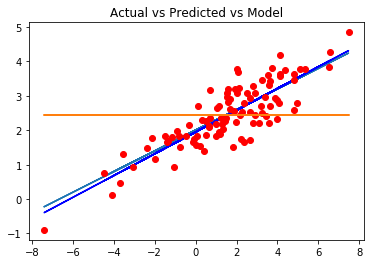
\includegraphics[width=10cm,keepaspectratio=true]{./images/optimalValue.png}
	% optimalValue.png: 0x0 pixel, 300dpi, 0.00x0.00 cm, bb=
\end{center}



Además del estadístico $R^{2}$, hay otras estadísticos y parámetros que uno necesita
mira para hacer lo siguiente:


\begin{enumerate}
	\item Seleccionar algunas variables y deseche otras para el modelo.
	
	
	\item Evaluar la relación entre el predictor y la variable de salida y verificar
	
	
	si una variable de predicción es significativa en el modelo o no.
	\item Calcular el error en los valores predichos por el modelo seleccionado.
\end{enumerate}




Veamos ahora algunas de los estadísticos que ayudan a abordar los Problemas
discutido anteriormente.

[]{Valor-$p$}
Es importante notar que al calcular los valores de $\a$ y $\beta,$ obtenemos estimados y no son exactos. Necesitamos demostrar su significación estadística usando una prueba de hipótesis.


La prueba de hipotética es acerca si el valor $\beta$ es diferente de cero o no. En otras palabras, si existe la correlación necesaria entre $X$ y $Y$. De haberla, $\beta \neq 0$.


En la ecuación $y = \a + \beta x,$ si hacemos $\beta=0,$ no existirá correlación entre $x$ y $y$. Entonces la prueba de hipótesis se define como
\begin{align}
	\texttt{Hipótesis Nula }H_{0}:\beta=0 \\
	\texttt{Hipótesis alternativa }H_{a}: \beta \neq 0
\end{align}




En general, si se realiza una regresión lineal y $\beta $ es calculado, este proceso estará acompañado por un estadístico$-t$ y el valor$-p$ correspondiente.



Como veremos más adelante, \texttt{Python} tiene implementado un método para calcular este valor$-p$.



Nuestra tarea entonces consistirá en comparar este valor$-p$ con un nivel dado de significación.



Como la desigualdad $\beta\neq 0$ se puede descomponer en dos desigualdades
\begin{align}
	\beta>0 \texttt{ o }\beta<0,
\end{align}
entonces será una prueba de dos colas, y si el valor$-p$ es menos que el nivel de significación, entonces la hipótesis nula $H_{0}: \beta = 0$ se rechaza y diremos que $\beta$ es significativo estadísticamente.



En caso contrario, nos permitirían no rechazar la hipótesis nula, de manera que $\beta$ sería, muy poco significativo estadísticamente.



Como veremos en el caso de una regresión múltiple, este hecho nos ayudará a omitir columnas innecesarias de nuestro modelo: Entre mayor sea el valor$-p,$ menos significativas serán para el modelo y viceversa.


[]{Estadístico$-F$}
Cuando uno se mueve de una regresión lineal simple a una regresión múltiple, existirán múltiples coeficientes $\beta$ y cada uno de estos indicará una estimación.



En tal caso, aparte de problemaar la significación de cada variable en particular en el modelo (revisando los valores$-p$ asociados con su estimador), también será necesario revisar si, como un grupo, todos los estimadores son significativos o no.




Esto se puede hacer de la siguiente manera:
\begin{align}
	\texttt{Hipótesis nula }& H_{0}:\beta_{1}=\beta_{2}=...=\beta_{n}=0 \\
	\texttt{Hipótesis alternativa }& H_{a}: \exists \beta_{i}\neq 0
\end{align}



El estadístico que se usa en esta prueba de hipótesis se llama \emph{estadístico$-F$} y se define de la siguiente manera:
\begin{align}
	F = \dfrac{\left( SST -SSD \right)/p}{SSD/\left( n-p-1 \right)}
\end{align}



Dicho estadístico sigue la distribución $F$.
Existirá un valor$-p$ asociado con este estadístico, tal que si dicho valor es suficientemente pequeño (es decir, menor al nivel de significación), la hipótesis nula puede ser rechazada.


[]

La significación del estadístico$-F$ es como sigue:
\begin{itemize}
	\item Los valores$-p$ son acerca de relaciones individuales entre un predictor y un resultado. En caso de más de un predictor, dicha relación puede cambiar debido a la presencia de otras variables.
	
	
	\item
	\emph{El estadístico$-F$ provee un manera de observar el cambio parcial en el valor$-p$ asociado debido a la adición de la nueva variable.}
	
	
	\item Cuando el número de los predictores en el modelos es muy grande y todas las $\beta_{i}\approx 0,$ los valores$-p$ individuales asociados con los predictores pueden ser muy pequeños.
	
	
	\item
	En tal caso, \emph{si sólo confiamos en valores$-p$ individuales, podríamos concluir incorrectamente que existe una relación entre los predictores y el resultado, cuando no es así en realidad, y debemos fijarnos en el valor$-p$ asociado con el estadístico$-F$.}
\end{itemize}



[, ]{Error residual estándar}

Otro concepto para aprender es el concepto de \emph{error residual estándar}.



Para un modelo de regresión lineal simple, se define de la siguiente manera:
\begin{align}
	RSE = \sqrt{\dfrac{1}{n-2}SSD}
\end{align}
donde $n$ es el número de datos puntuales.



En general,
\begin{align}
	RSE = \sqrt{\dfrac{SSD}{n-p-1}}
\end{align}
donde $p$ es el número de predictores en el modelo.



\texttt{RSE} es un estimado de la desviación estándar del término de error (\texttt{res}).


Este es el error que es inevitables aún si los coeficientes son conocidos correctamente.



Esto puede ser el caso porque el modelo carece de algo más, o quizá puede existir alguna variable en el modelo.



Nosotros sólo hemos mirado a una variable hasta ahora, pero en la mayoría de los escenarios tenemos que lidiar con regresiones múltiples, donde puede haber más de una variable de entrada.



En regresiones múltiples, los valores \texttt{RSE} tienden a disminuir, a medida que adicionamos más variables que son predictores más significativos de las variables de salida.




El valor \texttt{RSE} para un modelo puede ser calculado usando el siguiente pedazo de código. Aquí, estamos calculando \texttt{RSE} para el marco de datos que hemos usado en nuestro modelo, \texttt{df}:


[]{}
\begin{lstlisting}[language=Python]
	n = len(df['Input_Variable(X)'])
	df['SSD']=(df['Actual_Output(yact)']-df['ymodel'])**2
	SSD=df.sum()['SSD']
	RSE=np.sqrt(SSD/(n-2))
\end{lstlisting}



El valor \texttt{RSE} resultante en este caso es $\approx 0.4925$. Como se puede intuir, \emph{entre más pequeño sea \texttt{RSE}, mejor es el modelo}. Nuevamente, el punto de referencia para comparar este error es la media de los datos reales \texttt{yact}. Así que observaremos un error de $0.4925$ sobre $2.4512$, que es $\approx 20.09\%$ de error.

